\documentclass[11pt,a4paper]{article}

\usepackage[utf8]{inputenc}
\usepackage[francais]{babel}
\usepackage[T1]{fontenc}

\usepackage{graphicx}
\usepackage[margin=3cm]{geometry}
\usepackage{hyperref} %Pour les liens dans le sommaire
\usepackage{lscape} %Pour le format paysage
\usepackage{fancyhdr} %Pour le format du rapport
\usepackage{xcolor} %Pour l'utilisation de couleur dans le texte

\usepackage{amsmath}
\usepackage{amsfonts}
\usepackage{amssymb}


\definecolor{myGreen}{rgb}{0,0.46,0.38}
\definecolor{myKaki}{rgb}{0.60,0.45,0}
\definecolor{myBlue}{rgb}{0,0.45,0.68}
\definecolor{myPurple}{rgb}{0.51,0.25,0.76}
\definecolor{myOrange}{rgb}{0.95,0.50,0.05}
\definecolor{myDarkBlue}{rgb}{0,0,0.63}
\definecolor{myDarkRed}{rgb}{0.44,0,0}


\author{Théo DELACOUX - Adlane LADJAL}
\title{Devoir de MSI \\ Application Contagion}


\begin{document}

\makeatletter
\begin{titlepage}
	\centering
	\includegraphics[width=0.25\textwidth]{/Users/adlaneladjal/OneDrive/Etudes/logo_supgalilee.jpg}
	\hfill
	\includegraphics[width=0.25\textwidth]{/Users/adlaneladjal/OneDrive/Etudes/logo-paris13_bis.png} \\
    \vspace{5cm}
       {\LARGE \textbf{\@title}} \\
    \vspace{2em}
        {\large \@author }\\
    \vspace{1em}
        {\textit{\@date}} \\
    \vspace{2em}
    		
\includegraphics[width=0.25\textwidth]{contagion-logo.jpg}\\
    	\vspace{2em}
    		{Enseignant : John CHAUSSARD} \\
    \vfill
\end{titlepage}


%insertion de la page blanche
\newpage
~
\newpage

%Table des matieres
\renewcommand{\contentsname}{Sommaire}
\tableofcontents

\newpage

\pagestyle{empty}

\begin{landscape}
\section{Diagramme de cas d'utilisation}

\subsection{Le diagramme}

\vspace{1cm}

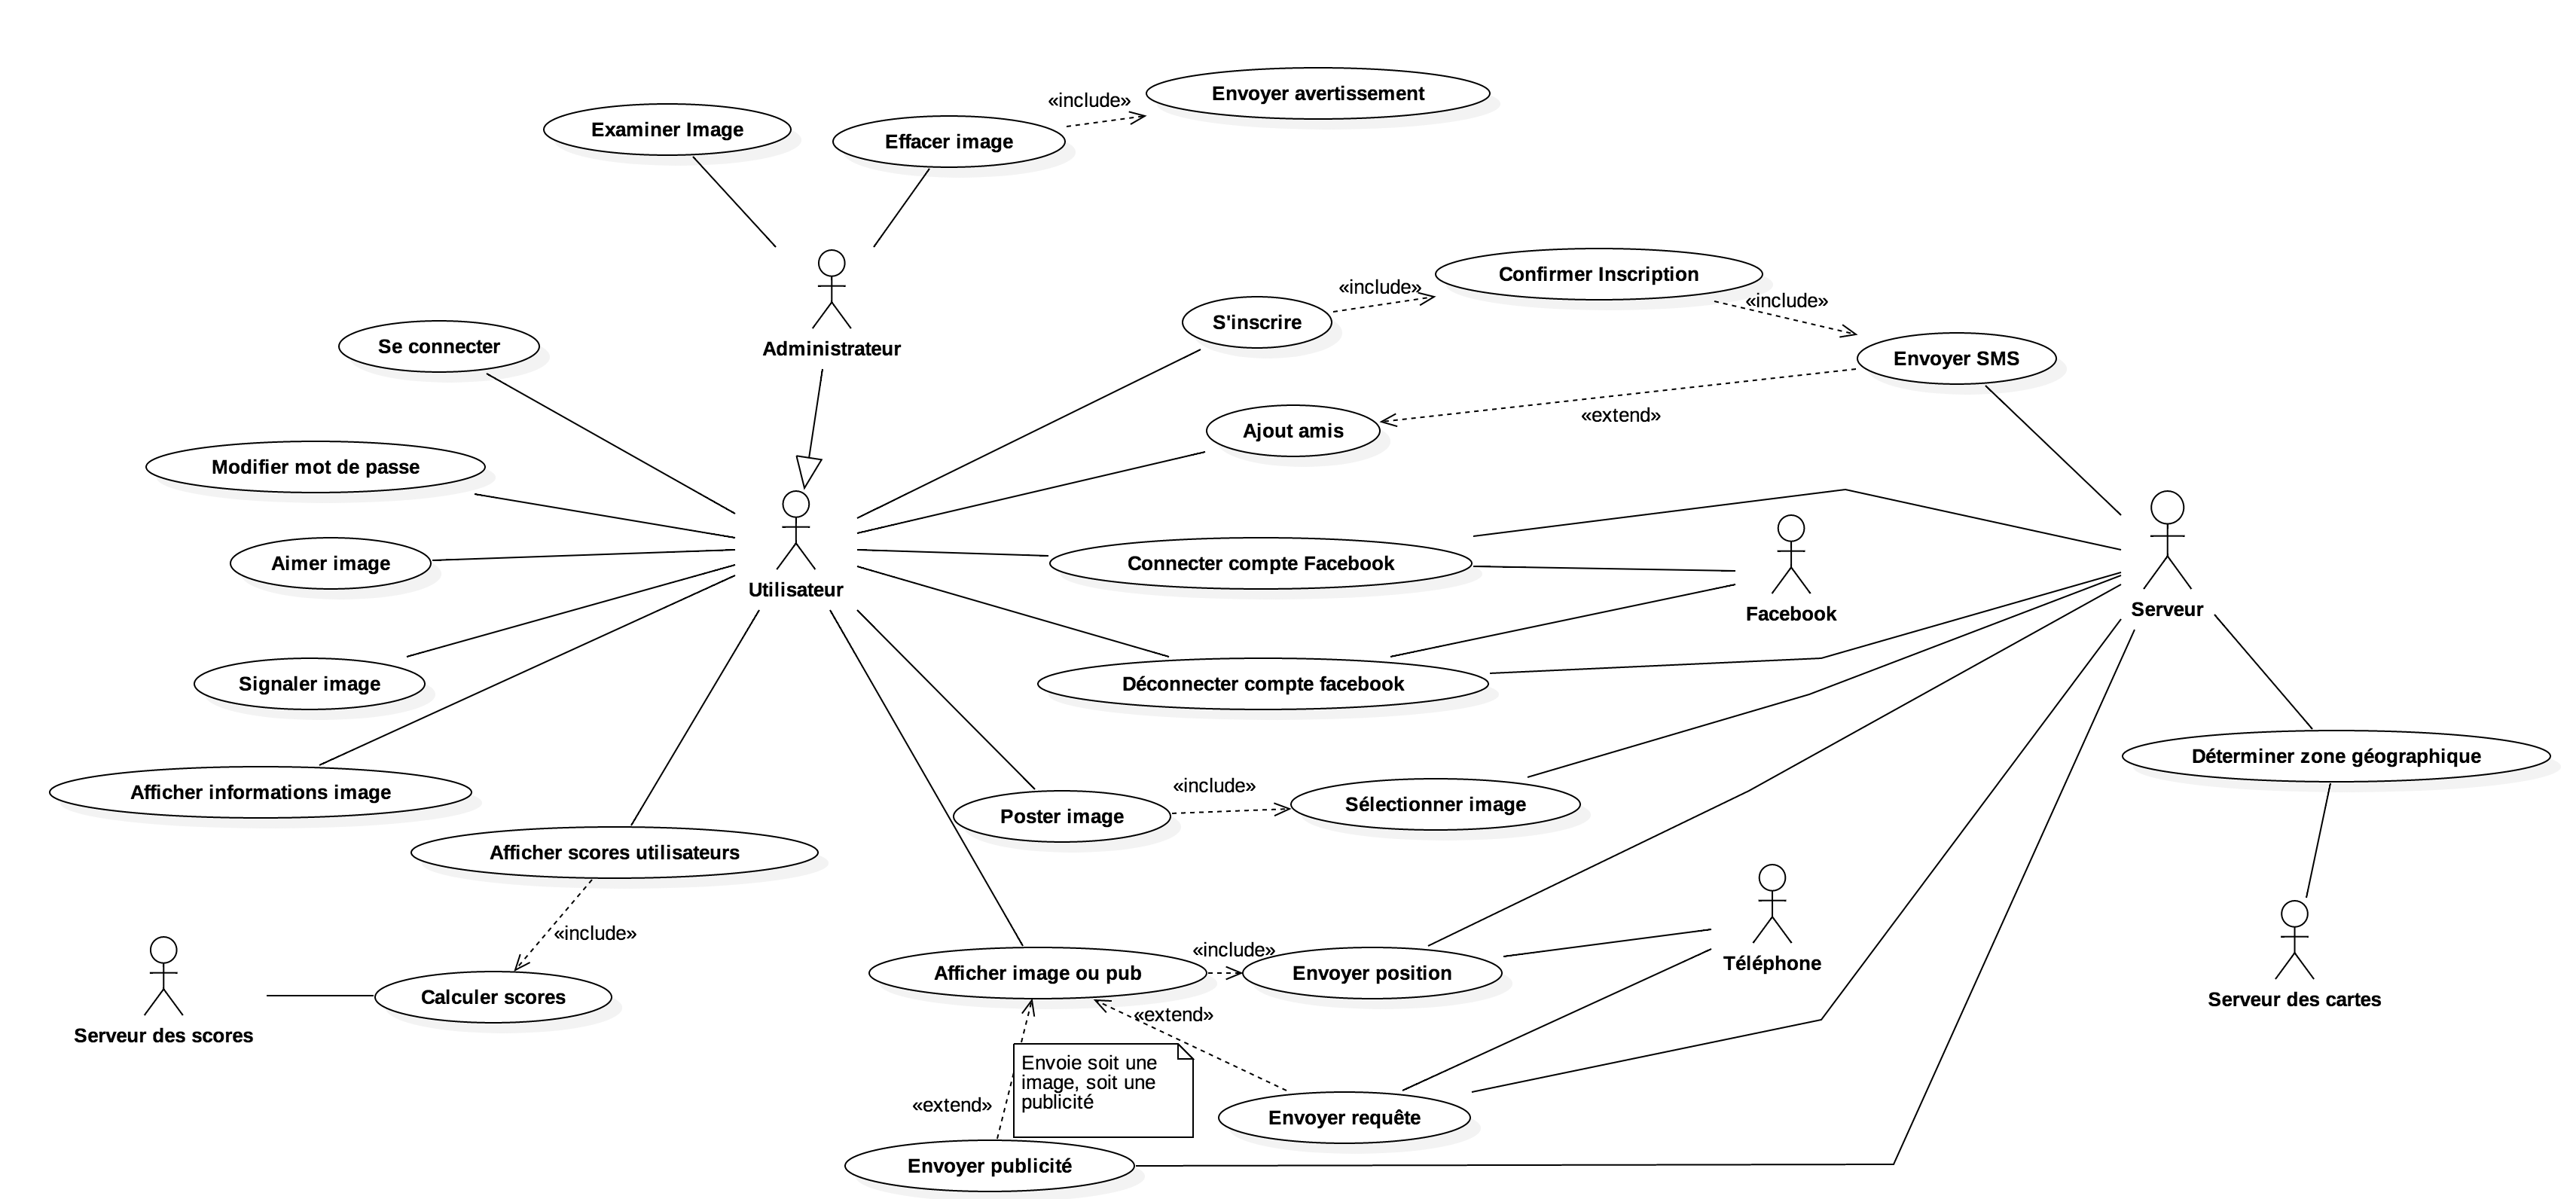
\includegraphics[scale=0.205]{/Users/adlaneladjal/OneDrive/Etudes/semestre6/MSI/Devoir/rendu/dcu.png}

\end{landscape}

\newpage

\pagestyle{fancy}
\fancyhead{}
\renewcommand{\headrulewidth}{0pt}

\subsection{Description}

Pour réaliser le diagramme de cas d’utilisation nous
avons fait le choix de prendre en compte un cadre d’étude
limité aux actions de l’utilisateur et du serveur. C’est
d’ailleurs nos deux principaux acteurs du diagramme. Nous
pouvons facilement le remarquer au vu du nombre de liens
que chacun détient.

\subsubsection{Les acteurs}

Nous avons identifié huit acteurs différents. Les voici : 

\begin{itemize}
	\item L’utilisateur
	\item L’administrateur
	\item Facebook
	\item Le téléphone
	\item Le serveur de Contagion
	\item Le serveur des cartes
	\item Le serveur des publicités
	\item Le serveur des scores
\end{itemize}

~\\

Plusieurs acteurs dans notre cadre d’étude sont qualifiés
de « serveur ». Mais nous n’avons pas de relation
d’héritage entre eux : ceci est dû, d’une part aux actions
trop différentes de chacun, mais aussi d’autre part, au
fait que le serveur des scores et le serveur des
publicités sont considérés externes à notre cadre d’étude.
Aussi, une relation d’héritage existe entre un
administrateur et un utilisateur. Nous avons considéré
qu’un administrateur avait la possibilité d’utiliser
l’application comme un utilisateur lambda. Seulement des
actions en plus lui sont conférés.

\subsubsection{Le cadre d'étude}
Nous avons plusieurs « sous »-cadre d’études distincts. Les voici avec leurs explications.

\paragraph{\textcolor{myGreen}{Informations de l’utilisateur et accession à l’application}}~\\
Pour qu’un utilisateur se connecte, il doit renseigner son
login et son mot de passe. Ce sont des cas d’utilisations
que nous avons choisi de ne pas représenter, en les
considérant comme implicites. Il en va de même pour le
formulaire à remplir lors de l’inscription. En revanche,
le fait de modifier est bien représenté car il est bien
distinct des deux autres citées plus tôt.

\paragraph{\textcolor{myKaki}{L'ajout d'amis}}~\\
L’utilisateur a la possibilité d’ajouter des amis de
plusieurs manières différentes. Nous avons choisi de ne
pas les représenter pour éviter de surcharger le
diagramme.

\paragraph{\textcolor{myBlue}{Compte Facebook}}~\\
Ici, nous n’avons pas représenté le fait que l’utilisateur
rentre son mot de passe et son login de son compte
Facebook. Nous avons en effet considéré que c’était des
cas d’utilisations propre à Facebook, qui sortaient alors
de notre cadre d’étude. En revanche, le fait de partager
une image peut venir de deux cas d’utilisations qui
appartiennent à la sous-section définie juste après.

\paragraph{\textcolor{myPurple}{Aimer et poster une image}}~\\
Aimer et poster une image sont des cas d’utilisations que
nous avons choisi de lier avec le cas « Partager une image
» de Facebook. En effet pour un utilisateur sont les seuls
moments où il peut interagir avec son compte Facebook.

\paragraph{\textcolor{myOrange}{Système d'affichage d'une image ou d'une publicité}}~\\
Lorsque l’utilisateur navigue sur l’application, il
affiche continuellement de nouvelles images. Or, le but de
l’application est d’afficher des images en fonction de sa
position. C’est alors par le téléphone, que le serveur
peut récupérer la position du téléphone, et donc celle de
l’utilisateur. Mais aussi, il se peut que le serveur
choisisse d’afficher une publicité (il doit alors
communiquer avec le serveur des publicités), à la place
d’une image. Donc finalement, un utilisateur apparaître
soit une image, soit une publicité sur son fil de
navigation ce qui explique la note. 

\paragraph{\textcolor{myDarkBlue}{Affichages d'informations sur une image}}~\\
Les informations d’une image appartiennent à la classe
image en elle-même dans notre représentation. Il n’y a
alors pas besoin de faire de requêtes auprès du serveur
pour avoir les informations sur une image. En revanche
pour calculer les scores, nous faisons appel à un serveur
externe : le serveur des scores.


\paragraph{\textcolor{myDarkRed}{Signalement d'une image}}~\\
S’il le souhaite l’utilisateur peut choisir de signaler
une image. C’est l’administrateur qui se charge de
l’examiner et de décider alors du sort de l’image.

\paragraph{Le cas d'utilisation « Envoyer SMS »}~\\
L’action d’envoyer un sms peut-être effectuer pour trois objectifs bien différents. Le premier pour envoyer une demande d’ami, le deuxième pour confirmer une inscription et le dernier pour prévenir un utilisateur de la censure de son image. Nous avons alors regroupé ces trois actions, pour une meilleure lisibilité. De plus pour ces trois objectifs, le serveur a un rôle à jouer.

\newpage

%%%%%%%%%%%%%%%%%%%%%%%%%%%%%%%%%%%%%%%%%%%%%%%%%%%%%%%%%

\section{Diagramme de classes}

\subsection{Le diagramme}
\subsection{Description}

\newpage

%%%%%%%%%%%%%%%%%%%%%%%%%%%%%%%%%%%%%%%%%%%%%%%%%%%%%%%%%

\section{Diagramme d'états-transitions}

\subsection{Le diagramme}

\vspace{4cm}

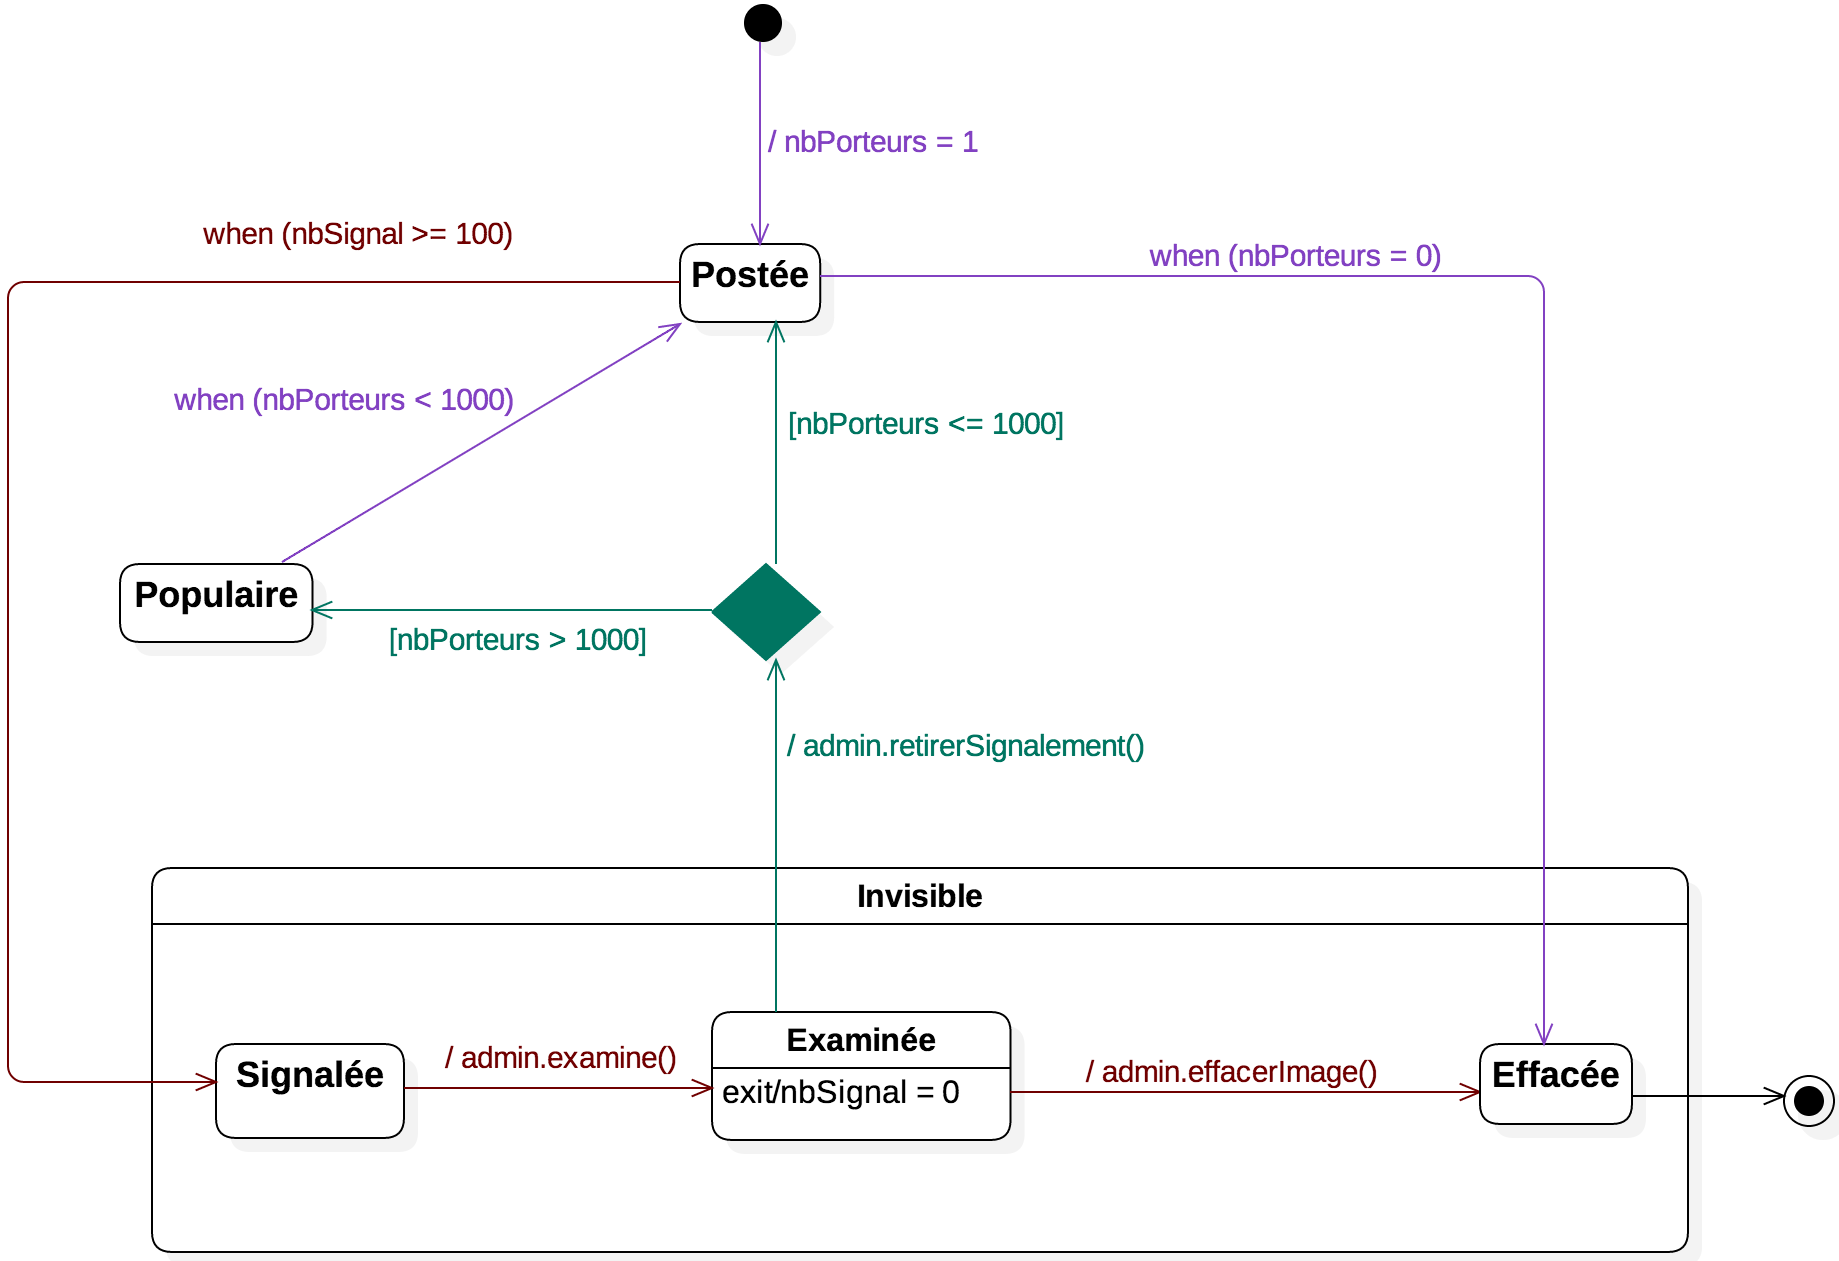
\includegraphics[scale=0.25]{/Users/adlaneladjal/OneDrive/Etudes/semestre6/MSI/Devoir/rendu/det.png}

\newpage

\subsection{Description}

Ce diagramme d’états-transitions représente les états que peut prendre une image sur le système.

\subsubsection{Les états}

\paragraph{Postée}~\\
Initialement, lorsqu’une image est postée, son nombre de 
porteur est initialisé à un : l’utilisateur qui a posté 
l’image.

\paragraph{Populaire}~\\
Nous avons considéré cet état comme un état à part
entière, car l’algorithme de sélection d’image de
Contagion va sortir une image populaire plus souvent
qu’une image qui ne l’est pas. Les paramètres d’une image
seront alors modifiés pour être plus facilement 
sélectionnée par cet algorithme. Il peut aussi y avoir 
plusieurs niveaux de popularité, que l’on aurait pu 
représenter sous la forme d’un état composite. Mais nous 
avons considéré qu’il était préférable de ne garder d’un 
niveau de popularité pour une meilleure compréhension.

\paragraph{Invisible}~\\
Ce cas d’utilisation n’est pas décrit dans l’énoncé. En
revanche nous avons jugé que cela peut-être une
fonctionnalité à rajouter. Lorsqu’une image est signalée
trop de fois, il est préférable de la rendre invisible aux
utilisateurs de Contagion.

\subparagraph{Signalée}
S’il y a beaucoup de signalements pour une image, cette
dernière rentre dans cet état.

\subparagraph{Examinée}
Puis un administrateur, examine l’image et décide de
l’action à effectuer : effacer l’image ou la juger
conforme aux Conditions Générales d’Utilisations.

\subparagraph{Effacée}
Dès qu’une image n’a plus de porteur (en effet un
utilisateur est porteur d’une image pendant une durée
finie selon l’énoncé), ou si un administrateur en a décidé
ainsi après signalement, elle est effacée.

~\\

\subsubsection{Les transitions}

Nous pouvons voir que les transitions, pour la plupart, 
portent des événements de type change, sur les nombres de 
signalements ou de porteurs. Ces nombres sont comparés aux 
valeurs 100 (pour le nombre de signalements) et 1 000 
(pour le nombre de porteurs). Ces valeurs ne sont 
qu’indicatives. Ils peuvent bien évidemment varier au 
cours du temps, être différent selon la zone géographique, 
selon l‘historique d’avertissements d’un utilisateur, etc… 
Ces comparaisons nous aident simplement à la meilleure 
compréhension du diagramme.\\
Les couleurs des transitions dépendent de la façon dont
elles sont réalisées.
\begin{itemize}
	\item \textcolor{myDarkRed}{Conditions sur le signalement.}
	\item \textcolor{myPurple}{Conditions sur le nombre de porteurs.}
	\item \textcolor{myGreen}{Cheminement lorsque le signalement d'une image est retirée.}
\end{itemize}




\end{document}
